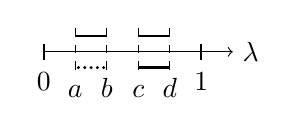
\begin{tikzpicture}[scale=2]

    % Axis
    \draw[->] (0,0) -- (1.2,0) node[right] {$\lambda$};

    % Tick marks and labels at 0 and 1
    \foreach \x/\label in {0/0, 1/1}
    {
        \draw[thick] (\x,0.05) -- (\x,-0.05);
        \node[below=4pt] at (\x,0) {$\label$};
    }

    % Two disjoint clusters
    \draw[thick] (0.2,0.1) -- (0.4,0.1);
    \draw[thick] (0.6,0.1) -- (0.8,0.1);
    % \node[above] at (0.3,0.1) {Cluster 1};
    % \node[above] at (0.7,0.1) {Cluster 2};
    % \node[left] at (0,0.1) {\small Two disjoint clusters};
    
    % Cluster with tail
    \draw[thick] (0.6,-0.1) -- (0.8,-0.1); % main cluster
    \foreach \x in {0.22,0.26,0.30,0.34,0.38} 
        \fill (\x,-0.1) circle (0.3pt); % tail eigenvalues
    % \node[below] at (0.7,-0.1) {Main cluster};
    % \node[below] at (0.3,-0.1) {Tail};
    % \node[left] at (0,-0.1) {\small Cluster with tail};
    
    % Mark points a, b, c, d
    \foreach \x/\label in {0.2/a, 0.4/b, 0.6/c, 0.8/d}
    {
        \draw[thin,dashed] (\x,0.15) -- (\x,-0.15);
        \node[above] at (\x,-0.35) {$\label$};
    }
    
\end{tikzpicture}